 % 3-Level Space Vector Modulation (SVM)
% Author: Amir Ostadrahimi


\documentclass [border=1pt]{standalone}
\usepackage{tikz}
\usepackage{xcolor} %package to define rgb colors
%define new colors
\definecolor{MatlabBlue}{rgb}{0 0.4470 0.7410} % define the blue color of the Matlab
\definecolor{MatlabBrown}{rgb}{0.8500 0.3250 0.0980} % define the brown color of the Matlab
\definecolor{MatlabYellow}{rgb}{0.9290 0.6940 0.1250} % define the yellow color of the Matlab
% define parameters
\newcommand\fillsize{1.5} %fillsaize= filling of the intersected vectors
\newcommand\Xone{1 cm} % x shift of the region name type 1
\newcommand\Yone{0.35 cm} %  y shift of the region name type 1
\newcommand\Ytwo{0.85 cm} %  y shift of the region name type 2
\newcommand\Vnamecolor{MatlabBlue} % vectron names color
\newcommand\Rnamecolor{MatlabBrown} %Region names color
\newcommand\axx{4.3} %axx= axis_x
\newcommand\axy{4.1} %axy= axis_y
%
\begin{document}
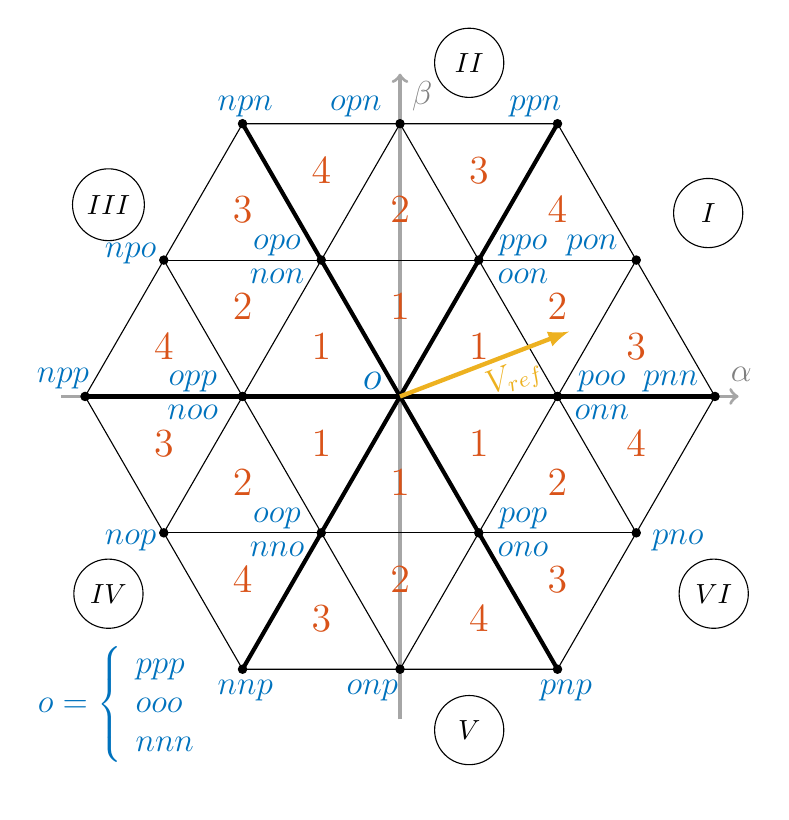
\begin{tikzpicture}
%coordinate
	\draw (0,0) coordinate (P0);
	\draw (P0)++(\axx,0) coordinate [ label={  [color=gray, xshift=1, yshift=2]  \large $\alpha$ }, color=gray!70] (P1){};
	\draw (P0)++(-\axx,0) coordinate (P2);
	\draw (P0)++(0,\axy) coordinate [label={[color=gray, xshift=8, yshift=-17] \large $\beta$ }] (P3)  {};
	\draw (P0)++(0,-\axy) coordinate(P4);
	\draw [->, very thick, color=gray!70] (P2)--(P1);
	\draw [->, very thick, color=gray!70] (P4)--(P3);
% Vectors
	%Large Vectors
	\draw  (0,0) -- (4,0) coordinate  [label={[MatlabBlue, xshift=-16, yshift=-2] \large $pnn$ }] (PNN) ;
	\filldraw [black] (PNN) circle (\fillsize pt);
	\draw (0,0) -- (2, 3.464) coordinate [label={[MatlabBlue, xshift=-8, yshift=-1] \large $ppn$ }](PPN) ;
	\filldraw [black] (PPN) circle (\fillsize pt);
	\draw  (0,0) -- (-2, 3.464) coordinate[label={[MatlabBlue, xshift=1, yshift=-1]\large $npn$ }] (NPN)  ;
	\filldraw [black] (NPN) circle (\fillsize pt);
	\draw  (0,0) -- (-4,0) coordinate [label={[MatlabBlue, xshift=-8, yshift=-1] \large $npp$ }] (NPP);
	\filldraw [black] (NPP) circle (\fillsize pt);
	\draw  (0,0) -- (-2, -3.464) coordinate [label={[MatlabBlue, xshift=1, yshift=-15] \large $nnp$ }] (NNP) ;
	\filldraw [black] (NNP) circle (\fillsize pt);
	\draw  (0,0) -- (2, -3.464) coordinate [label={[MatlabBlue, xshift=3, yshift=-15] \large $pnp$ }] (PNP) ;
	\filldraw [black] (PNP) circle (\fillsize pt);
	%Medium Vectors
	\draw (0,0) ++ (3, 1.732) coordinate [label={[MatlabBlue, xshift=-16, yshift=-2] \large $pon$ }] (PON) {} ;
	\filldraw [black] (PON) circle (\fillsize pt);
	\draw  (0,0)++ (0, 3.464) coordinate [label={[MatlabBlue, xshift=-16, yshift=-1]  \large $opn$ }] (OPN) {} ;
	\filldraw [black] (OPN) circle (\fillsize pt);
	\draw  (0,0) ++ (-3, 1.732) coordinate [label={[MatlabBlue, xshift=-12, yshift=-5] \large $npo$ }] (NPO) {} ;
	\filldraw [black] (NPO) circle (\fillsize pt);
	\draw (0,0) ++ (-3, -1.732) coordinate [label={[MatlabBlue, xshift=-12, yshift=-10] \large $nop$ }] (NOP) {} ;
	\filldraw [black] (NOP) circle (\fillsize pt);
	\draw  (0,0) ++ (0, -3.464) coordinate [label={[MatlabBlue, xshift=-10, yshift=-15] \large $onp$ }] (ONP) {} ;
	\filldraw [black] (ONP) circle (\fillsize pt);
	\draw  (0,0) ++ (3, -1.732) coordinate [label={[MatlabBlue, xshift=15, yshift=-10] \large $pno$ }] (PNO) {} ;
	\filldraw [black] (PNO) circle (\fillsize pt);
	%Small Vectors
	\draw  (0,0) ++ (2,0) coordinate  [label={[MatlabBlue, xshift=16, yshift=-2] \large $poo$ }] (POO) ;
	\draw  (0,0) ++ (2,0) coordinate  [label={[MatlabBlue, xshift=16, yshift=-12] \large $onn$ }] (ONN) ;
	\filldraw [black] (ONN) circle (\fillsize pt);
	\draw  (0,0)++ (1, 1.732) coordinate [label={[MatlabBlue, xshift=16, yshift=-2] \large $ppo$ }](PPO) ;
	\draw  (0,0) ++ (1, 1.732) coordinate [label={[MatlabBlue, xshift=16, yshift=-12] \large $oon$ }](OON) ;
	\filldraw [black] (OON) circle (\fillsize pt);
	\draw  (0,0) ++ (-1, 1.732) coordinate[label={[MatlabBlue, xshift=-16, yshift=-2]\large $opo$ }] (OPO)  ;
	\draw  (0,0) ++ (-1, 1.732) coordinate[label={[MatlabBlue, xshift=-16, yshift=-12]\large $non$ }] (NON)  ;
	\filldraw [black] (NON) circle (\fillsize pt);
	\draw  (0,0) ++ (-2,0) coordinate [label={[MatlabBlue, xshift=-18, yshift=-2] \large $opp$ }] (OPP);
	\draw (0,0)++ (-2,0) coordinate [label={[MatlabBlue, xshift=-18, yshift=-12] \large $noo$ }] (NOO);
	\filldraw [black] (NOO) circle (\fillsize pt);
	\draw (0,0)++ (-1, -1.732) coordinate [label={[MatlabBlue, xshift=-16, yshift=-2] \large $oop$ }] (OOP) ;
	\draw (0,0) ++ (-1, -1.732) coordinate [label={[MatlabBlue, xshift=-16, yshift=-12] \large $nno$ }] (NNO) ;
	\filldraw [black] (NNO) circle (\fillsize pt);
	\draw  (0,0) ++ (1, -1.732) coordinate [label={[MatlabBlue, xshift=16, yshift=-2] \large $pop$ }] (POP) ;
	\draw  (0,0) ++  (1, -1.732) coordinate [label={[MatlabBlue, xshift=16, yshift=-12] \large $ono$ }] (ONO) ;
	\filldraw [black] (ONO) circle (\fillsize pt);
	% Zero Vector
	\filldraw [black] (P0) circle (\fillsize pt);
	\draw  (0,0)  coordinate [label={[MatlabBlue, xshift=-10, yshift=-1] \Large $o$ }] (PPP) ;
	\node  (OOO) at (-3.5, -4.9) [ label={[MatlabBlue, align=left]\large $ o=\left\{ \begin{array}{ll}ppp\\ooo \\nnn
	    \end{array} \right. $} ] {};
% LINES
	%Surrounding lines
	\draw  (PNN)--(PPN)--(NPN)--(NPP)--(NNP)--(PNP)--(PNN);
	%-orizontal lines
	\draw  (PON)--(PPO)--(OPO)--(NPO);
	\draw  (PNO)--(POP)--(OOP)--(NOP);
	%Oblique lines
	%Starting from opn
	\draw  (OPN)--(PPO)--(POO)--(PNO);
	\draw (OPN)--(OPO)--(OPP)--(NOP);
	%starting from onp
	\draw  (ONP)--(POP)--(POO)--(PON);
	\draw  (ONP)--(OOP)--(OPP)--(NPO);
% SECTOR
	% bold lines for sectors
	\draw  [line width=1.5pt] (P0)--(PNN);
	\draw  [line width=1.5pt] (P0)--(PPN);
	\draw  [line width=1.5pt] (P0)--(NPN);
	\draw  [line width=1.5pt] (P0)--(NPP);
	\draw  [line width=1.5pt] (P0)--(NNP);
	\draw  [line width=1.5pt] (P0)--(PNP);
	%Sector numbers
	\node [  xshift=26, yshift=17, circle,draw, minimum size =25] (SEC1) at (PON) { $I$};
	\node [  xshift=25, yshift=22, circle,draw, minimum size =25]  (SEC2) at (OPN) {$II$};%%
	\node [  xshift=-20, yshift=20, circle,draw, minimum size =25]  (SEC3) at (NPO) { $III$};
	\node [  xshift=-20, yshift=-22, circle,draw, minimum size =25]  (SEC4) at (NOP) {$IV$};
	\node [ xshift=25, yshift=-22, circle,draw,minimum size =25]  (SEC5) at (ONP) {$V$};%%
	\node [ xshift=28, yshift=-22, circle,draw, minimum size =25]  (SEC6) at (PNO) { $VI$};
%Region numbers
	%Sector 1
	\coordinate  [label={[\Rnamecolor, xshift=\Xone, yshift=\Yone]  \Large $1$ }] (S1-1) at (P0); %R1
	\coordinate  [label={[\Rnamecolor, xshift=0, yshift=\Ytwo]  \Large  $2$ }] (S1-2) at (POO); %R2
	\coordinate  [label={[\Rnamecolor,xshift=\Xone , yshift=\Yone]   \Large$3$ }] (S1-3) at (POO); %R3
	\coordinate  [label={[\Rnamecolor, xshift=\Xone, yshift=\Yone]   \Large $4$ }] (S1-4) at (PPO); %R4
	%Sector 2
	\coordinate  [label={[\Rnamecolor, xshift=0, yshift=\Ytwo]  \Large $1$ }] (S2-1) at (P0); %R1
	\coordinate  [label={[\Rnamecolor, xshift=\Xone, yshift=\Yone]  \Large  $2$ }] (S2-2) at (OPO); %R2
	\coordinate  [label={[\Rnamecolor, xshift=0, yshift=\Ytwo]   \Large$3$ }] (S2-3) at (PPO); %R3
	\coordinate  [label={[\Rnamecolor, xshift=0, yshift=\Ytwo]   \Large $4$ }] (S2-4) at (OPO); %R4
	%Sector 3
	\coordinate  [label={[\Rnamecolor, xshift=\Xone, yshift=\Yone]  \Large $1$ }] (S3-1) at (OPP); %R1
	\coordinate  [label={[\Rnamecolor, xshift=0, yshift=\Ytwo]  \Large  $2$ }] (S3-2) at (OPP); %R2
	\coordinate  [label={[\Rnamecolor,xshift=\Xone , yshift=\Yone]   \Large$3$ }] (S3-3) at (NPO); %R3
	\coordinate  [label={[\Rnamecolor, xshift=\Xone, yshift=\Yone]   \Large $4$ }] (S3-4) at (NPP); %R4
	%Sector 4
	\coordinate  [label={[\Rnamecolor, xshift=0, yshift=\Ytwo]  \Large $1$ }] (S4-1) at (OOP); %R1
	\coordinate  [label={[\Rnamecolor, xshift=\Xone, yshift=\Yone]  \Large  $2$ }] (S4-2) at (NOP); %R2
	\coordinate  [label={[\Rnamecolor, xshift=0, yshift=\Ytwo]   \Large$3$ }] (S4-3) at (NOP); %R3
	\coordinate  [label={[\Rnamecolor, xshift=0, yshift=\Ytwo]   \Large $4$ }] (S4-4) at (NNP); %R4
	%Sector 5
	\coordinate  [label={[\Rnamecolor, xshift=\Xone, yshift=\Yone]  \Large $1$ }] (S5-1) at (OOP); %R1
	\coordinate  [label={[\Rnamecolor, xshift=0, yshift=\Ytwo]  \Large  $2$ }] (S5-2) at (ONP); %R2
	\coordinate  [label={[\Rnamecolor,xshift=\Xone , yshift=\Yone]   \Large$3$ }] (S5-3) at (NNP); %R3
	\coordinate  [label={[\Rnamecolor, xshift=\Xone, yshift=\Yone]   \Large $4$ }] (S5-4) at (ONP); %R4
	%Sector 4
	\coordinate  [label={[\Rnamecolor, xshift=0, yshift=\Ytwo]  \Large $1$ }] (S6-1) at (POP); %R1
	\coordinate  [label={[\Rnamecolor, xshift=\Xone, yshift=\Yone]  \Large  $2$ }] (S6-2) at (POP); %R2
	\coordinate  [label={[\Rnamecolor, xshift=0, yshift=\Ytwo]   \Large$3$ }] (S6-3) at (PNP); %R3
	\coordinate  [label={[\Rnamecolor, xshift=0, yshift=\Ytwo]   \Large $4$ }] (S6-4) at (PNO); %R4
%-Reference vector
\draw [MatlabYellow, line width=0.55 mm, -latex] (P0)--++(21:2.3) coordinate [label={[MatlabYellow, xshift=-16, yshift=-26,rotate=21]  \large $V_{ref}$ }] (Vref);
\end{tikzpicture}
\end{document} 


